После начала нагрева с помощью вольтметра и термопары снимем температурную зависимость проводимости меди и полупроводника (см. таблицу 1, приложение). Так как для полупроводника достаточно быстро меняется $R$, примем относительную погрешность измерения равной 2 \%. Пересчитаем сопротивления в $\sigma$, расчитаем погрешность и занесем данные в таблицу.


Построим линеаризованную зависимость $\ln(\sigma/\sigma_0)[1/T] = a / T + b$ для полупроводника и линеаризованную зависимость $\sigma/\sigma_0 [1/T] = \alpha /T + \beta$ для меди (рис. 2). Значения $\xi^2/\text{ndf}$ указаны на графиках. 

\begin{figure}[h]
    \centering
    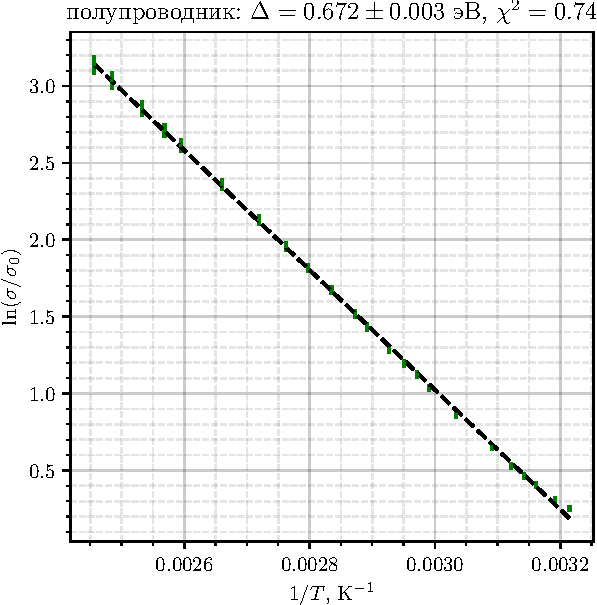
\includegraphics[width=0.45\textwidth]{plot_sc_6.11.1.pdf}
    \hspace{5 mm} 
    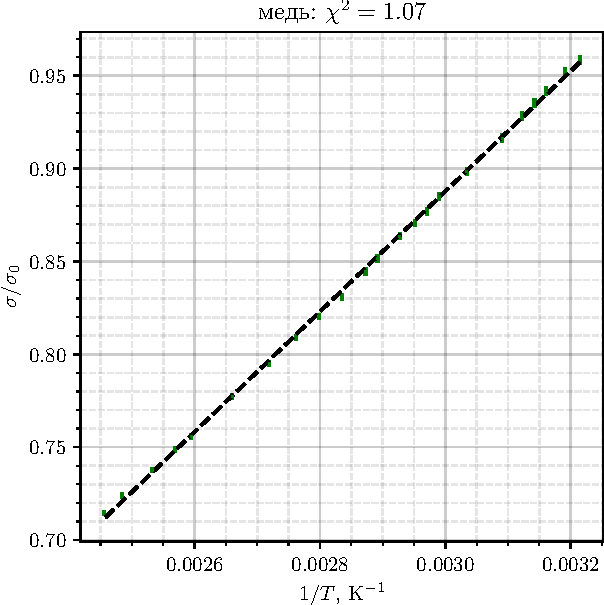
\includegraphics[width=0.45\textwidth]{plot_cu_6.11.1.pdf}
    \caption{Линеаризованная зависимость проводимости от температуры для полупроводника и меди}
    \label{fig:sccu}
\end{figure}

Для меди $\alpha = (324 \pm 2) \text{ К}^{-1}$, с $\sigma_0 = 5.7  \times  10^7 \text{ Ом}^{-1} \text{м}$, что вполне согласется с табличным значением для удельного сопротивления  $\Delta \rho / \Delta T = 4.1 \times 10^{-3} \text{К}^{-1}$.

По линеаризованной зависимости найдём
\begin{equation*}
    a = -(3.90 \pm 0.2) \times 10^3 \text{ К}^{-1},
    \hspace{0.5cm} \Rightarrow \hspace{0.5cm} 
    \Delta = - 2 k a = (0.672 \pm 0.003) \text{ эВ},
\end{equation*}
что очень близко к величине запрещенной зоны германия $\sub{\Delta}{Ge} = 0.67$ эВ.



\subsection*{Вывод}


Измерена зависимость проводимости металла (меди) и полупроводника от температуры. С $\chi^2 \sim 1$ данные согласуются с линейной зависимостью от обратной температуры для металла и экспоненциальной для полупроводника. 

Найдена ширина запрещенной зоны для полупроводника $\Delta = (0.672 \pm 0.003)$ эВ, соответствующая табличному значению.
